\begin{problem}{/images/problems/52_pic.jpg}{Non-isomorphic Graphs}  There are $2^{10}$ undirected unweighted graphs with 5 vertices. Two graphs are called isomorphic, if one can obtain one of them by changing the labels of the vertices of the other graph. An example of two isomorphic graphs is given in the figure below.

\begin{center}
	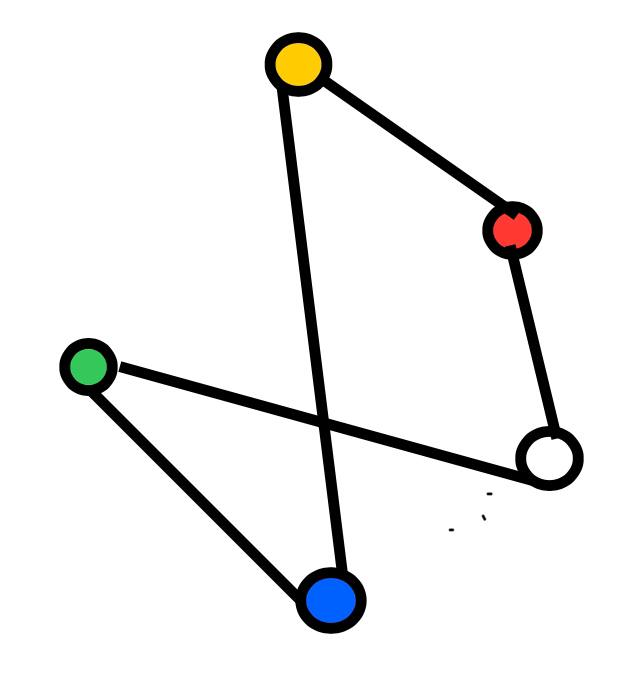
\includegraphics[width=4cm]{/images/problems/52_p1.jpg}	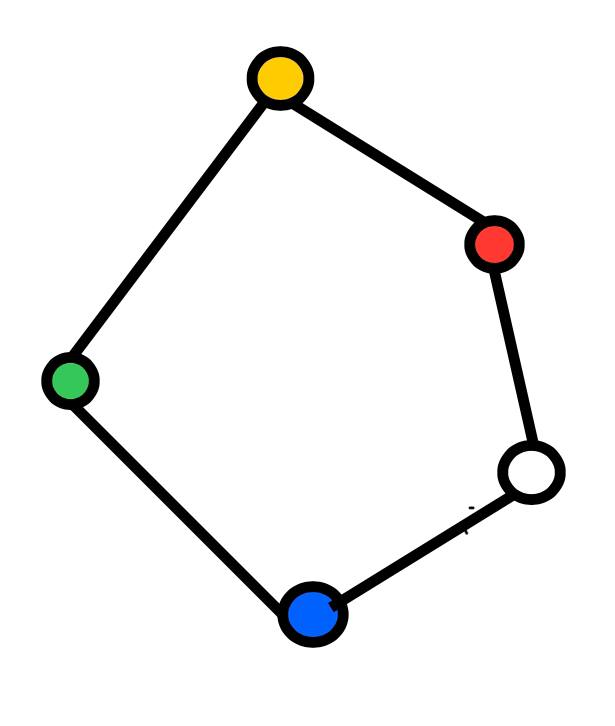
\includegraphics[width=4cm]{/images/problems/52_p2.jpg}
\end{center}	

Solve the following problem without using a computer: How many non-isomorphic unweighted undirected graphs with 5 vertices are there?
\end{problem}
\begin{solution}
The solution is equal to $34$.\\[0.2cm]

From here on, when we use the term a graph with $n$ vertices, we mean an unweighted undirected graph with vertices labelled with $1, 2, 3, \ldots, n$. Let $G$ be a graph with $n$ vertices and $P = \langle p_1, p_2, \ldots, p_n \rangle$ be a permutation of numbers $1$ to $n$. We define the transformation of $G$ by permutation $P$ as a graph identical to $G$ with the exception that the label of each vertex $i$ is replaced by $p_i$. We denote this transformation by $T(G, P)$.
We use the following lemma to count the number of non-isomorphic graphs with 5 vertices. We defer the proof of the lemma to the end of the solution.
\begin{lemma}\label{lemma:1}
	For a given $n$, let $x_n$ be the number of pairs $(G, P)$ such that $G$ is a graph with $n$ vertices, $P$ is  permutation of numbers $1,2, \ldots, n$, and $T(G, P) = G$. The number of non-isomorphic graphs with $n$ vertices is equal to $x_n/n!$.
\end{lemma}


Based on Lemma~\ref{lemma:1}, the answer to this question is equal to $x_5 / 120$. Thus, our aim is to find the value of $x_5$.\\[0.2cm]

We can categorize the permutations of numbers $1, 2, \ldots, n$ by the length of the cycles of their permutation graph:
\begin{itemize}
	\item 5 cycles of size 1: $\langle 1, 2, 3, 4 ,5 \rangle$ is the only permutations whose permutation graph has 5 cycles. All the $2^{10}$ graphs with 5 vertices will remain intact under this permutation.
	\item 3 cycles of size 1 and 1 cycle of size 2: There are $\binom{5}{2} = 10$ permutations whose permutation graphs have 3 cycles of size 1 and 1 cycle of size 2. $2^{7}$ graphs with 5 vertices will remain intact under such  permutations.
	\item 2 cycles of size 1 and 1 cycle of size 3: There are $2\binom{5}{3} = 20$ permutations whose permutation graphs have 2 cycles of size 1 and one cycle of size 3. $2^{4}$ graphs with 5 vertices will remain intact under such  permutations
	\item 1 cycle of size 1 and 1 cycle of size $4$: There are $6\binom{5}{4} = 30$ permutations whose permutation graphs have 1 cycle of size 1 and 1 cycle of size 4. $2^{3}$ graphs with 5 vertices will remain intact under such  permutations
	\item 1 cycle of size 2 and 1 cycle of size 3: There are $2\binom{5}{3} = 20$ permutations whose permutation graphs have 1 cycle of size 2 and 1 cycle of size 3. $2^{3}$ graphs with 5 vertices will remain intact under such  permutations
	\item 1 cycle of size 1 and 2 cycles of size 2: There are $\binom{5}{2} \binom{3}{2}/2 = 15$ permutations whose permutation graphs have 1 cycle of size 1 and two cycles of size 2. $2^{6}$ graphs with 5 vertices will remain intact under such  permutations
	\item 1 cycle of size 5: There are $4! = 24$ permutations whose permutation graphs have 1 cycle of size 5. There are 4 graphs with 5 vertices will remain intact under such  permutations.
\end{itemize}
Therefore, $x_5 = 2^{10} + 10\cdot 2^7 + 20\cdot 2^4 + 30\cdot 2^3 + 20\cdot 2^3 + 15\cdot 2^6 + 4!\cdot 4 = 4080$. Thus, the answer is equal to $4080/120 = 34$.\\[0.2cm]

\begin{proof}[Proof of Lemma~\ref{lemma:1}]
	Consider a super graph with $2^{\binom{n}{2}}$ vertices, each corresponding to a graph with $n$ vertices. For each permutation $P$, we draw an edge between vertex $u$ and vertex $v$ with label $P$ if $T(u) = v$. The number of non-isomorphic graphs with $n$ vertices is equal to the number of connected components of this super graph. Notice that the degrees of all vertices of the super graph are equal to $n!$. Moreover, all   vertices of each connected component represent isomorphic graphs. This means that for each connected component, the number of edges between every pair of vertices are the same, and this value is equal to the number of loops of each vertex within the component. Thus, the summation of the number of loops of the vertices in each component is equal to $n!$. This implies that the total number of loops over $n!$ is the number of components of the super graph which is equal to the number of non-isomorphic graphs of size $n$.
\end{proof}
\end{solution}
